\documentclass{sigchi}

% Use this section to set the ACM copyright statement (e.g. for
% preprints).  Consult the conference website for the camera-ready
% copyright statement.

% Copyright
\CopyrightYear{2016}
%\setcopyright{acmcopyright}
\setcopyright{acmlicensed}
%\setcopyright{rightsretained}
%\setcopyright{usgov}
%\setcopyright{usgovmixed}
%\setcopyright{cagov}
%\setcopyright{cagovmixed}
% DOI
\doi{http://dx.doi.org/10.475/123_4}
% ISBN
\isbn{123-4567-24-567/08/06}
%Conference
\conferenceinfo{CHI'16,}{May 07--12, 2016, San Jose, CA, USA}
%Price
\acmPrice{\$15.00}

% Use this command to override the default ACM copyright statement
% (e.g. for preprints).  Consult the conference website for the
% camera-ready copyright statement.

%% HOW TO OVERRIDE THE DEFAULT COPYRIGHT STRIP --
%% Please note you need to make sure the copy for your specific
%% license is used here!
% \toappear{
% Permission to make digital or hard copies of all or part of this work
% for personal or classroom use is granted without fee provided that
% copies are not made or distributed for profit or commercial advantage
% and that copies bear this notice and the full citation on the first
% page. Copyrights for components of this work owned by others than ACM
% must be honored. Abstracting with credit is permitted. To copy
% otherwise, or republish, to post on servers or to redistribute to
% lists, requires prior specific permission and/or a fee. Request
% permissions from \href{mailto:Permissions@acm.org}{Permissions@acm.org}. \\
% \emph{CHI '16},  May 07--12, 2016, San Jose, CA, USA \\
% ACM xxx-x-xxxx-xxxx-x/xx/xx\ldots \$15.00 \\
% DOI: \url{http://dx.doi.org/xx.xxxx/xxxxxxx.xxxxxxx}
% }

% Arabic page numbers for submission.  Remove this line to eliminate
% page numbers for the camera ready copy
% \pagenumbering{arabic}

% Load basic packages
\usepackage{balance}       % to better equalize the last page
\usepackage{graphics}      % for EPS, load graphicx instead 
\usepackage[T1]{fontenc}   % for umlauts and other diaeresis
\usepackage{txfonts}
\usepackage{mathptmx}
\usepackage[pdflang={en-US},pdftex]{hyperref}
\usepackage{color}
\usepackage{booktabs}
\usepackage{textcomp}

% Some optional stuff you might like/need.
\usepackage{microtype}        % Improved Tracking and Kerning
% \usepackage[all]{hypcap}    % Fixes bug in hyperref caption linking
\usepackage{ccicons}          % Cite your images correctly!
% \usepackage[utf8]{inputenc} % for a UTF8 editor only

% If you want to use todo notes, marginpars etc. during creation of
% your draft document, you have to enable the "chi_draft" option for
% the document class. To do this, change the very first line to:
% "\documentclass[chi_draft]{sigchi}". You can then place todo notes
% by using the "\todo{...}"  command. Make sure to disable the draft
% option again before submitting your final document.
\usepackage{todonotes}

% Paper metadata (use plain text, for PDF inclusion and later
% re-using, if desired).  Use \emtpyauthor when submitting for review
% so you remain anonymous.
\def\plaintitle{Evaluating the Effect of Induced Synesthesia in Learning a Musical Skill}
\def\plainauthor{First Author, Second Author, Third Author,
  Fourth Author, Fifth Author, Sixth Author}
\def\emptyauthor{}
\def\plainkeywords{Authors' choice; of terms; separated; by
  semicolons; include commas, within terms only; required.}
\def\plaingeneralterms{Documentation, Standardization}

% llt: Define a global style for URLs, rather that the default one
\makeatletter
\def\url@leostyle{%
  \@ifundefined{selectfont}{
    \def\UrlFont{\sf}
  }{
    \def\UrlFont{\small\bf\ttfamily}
  }}
\makeatother
\urlstyle{leo}

% To make various LaTeX processors do the right thing with page size.
\def\pprw{8.5in}
\def\pprh{11in}
\special{papersize=\pprw,\pprh}
\setlength{\paperwidth}{\pprw}
\setlength{\paperheight}{\pprh}
\setlength{\pdfpagewidth}{\pprw}
\setlength{\pdfpageheight}{\pprh}

% Make sure hyperref comes last of your loaded packages, to give it a
% fighting chance of not being over-written, since its job is to
% redefine many LaTeX commands.
\definecolor{linkColor}{RGB}{6,125,233}
\hypersetup{%
  pdftitle={\plaintitle},
% Use \plainauthor for final version.
%  pdfauthor={\plainauthor},
  pdfauthor={\emptyauthor},
  pdfkeywords={\plainkeywords},
  pdfdisplaydoctitle=true, % For Accessibility
  bookmarksnumbered,
  pdfstartview={FitH},
  colorlinks,
  citecolor=black,
  filecolor=black,
  linkcolor=black,
  urlcolor=linkColor,
  breaklinks=true,
  hypertexnames=false
}

% create a shortcut to typeset table headings
% \newcommand\tabhead[1]{\small\textbf{#1}}

% End of preamble. Here it comes the document.
\begin{document}

\title{\plaintitle}

\numberofauthors{5}
\author{%
  \alignauthor{Kevin Key\\
	\affaddr{MS-HCI, Augmented Reality}\\
	\affaddr{Georgia Institute of Technology}\\
    \affaddr{Atlanta, GA}\\
    \email{key@gatech.com}}\\
  \alignauthor{Sumedha Raman\\
	\affaddr{MSCS Interactive Intelligence}\\
	\affaddr{Georgia Institute of Technology}\\
    \affaddr{Atlanta, GA}\\
    \email{sraman46@gatech.edu}}\\
  \alignauthor{Russell Strauss\\
	\affaddr{MSCS Computer Graphics}\\
	\affaddr{Georgia Institute of Technology}\\
    \affaddr{Atlanta, GA}\\
    \email{russellstrauss@gatech.edu}}\\
  \alignauthor{Rikesh Subedi\\
	\affaddr{BS Computer Science}\\
	\affaddr{Georgia Institute of Technology}\\
    \affaddr{Atlanta, GA}\\
    \email{rsubedi3@gatech.edu}}\\
  \alignauthor{Santiago Arconada\\
	\affaddr{MS-HCI}\\
	\affaddr{Georgia Institute of Technology}\\
    \affaddr{Atlanta, GA}\\
    \email{sarconada@gatech.edu}}\\
}

\maketitle

\begin{abstract}
	This study involves the simulation of a synesthesia-like experience for non-synesthetes, to enhance the learning of a musical skill. The goal of this project is to validate whether a synesthesia-like experience could positively influence the acquisition of musical talent. The idea is to increase the number of associations made to a chord (a harmonic group of notes). In this work, chord-color mappings are manifested using colored visuals displayed while listening to music. The expected outcome is that students who learn using consistent chord-color associations will perform better when tested on the identification of chords.
\end{abstract}

\section{Introduction}

Synesthesia is a condition of the human mind where seemingly unrelated senses are experienced simultaneously [1]. An example of this is seeing color when you hear sound or seeing written words and numbers in color. The current data shows that 2\% of the population has some degree of this condition, with a larger concentration in artistic communities. This suggests that there is a correlation between creative skill and sensory experience. Synesthetes have a biological advantage which makes them more receptive to early exploration and adoption thus translating into more expertise in adulthood.




% Use a numbered list of references at the end of the article, ordered
% alphabetically by first author, and referenced by numbers in
% brackets~\cite{ethics, Klemmer:2002:WSC:503376.503378,
%   Mather:2000:MUT, Zellweger:2001:FAO:504216.504224}. For papers from
% conference proceedings, include the title of the paper and an
% abbreviated name of the conference (e.g., for Interact 2003
% proceedings, use \textit{Proc. Interact 2003}). Do not include the
% location of the conference or the exact date; do include the page
% numbers if available. See the examples of citations at the end of this
% document. Within this template file, use the \texttt{References} style
% for the text of your citation.

% Your references should be published materials accessible to the
% public.  Internal technical reports may be cited only if they are
% easily accessible (i.e., you provide the address for obtaining the
% report within your citation) and may be obtained by any reader for a
% nominal fee.  Proprietary information may not be cited. Private
% communications should be acknowledged in the main text, not referenced
% (e.g., ``[Robertson, personal communication]'').

% \begin{figure*}
%   \centering
%   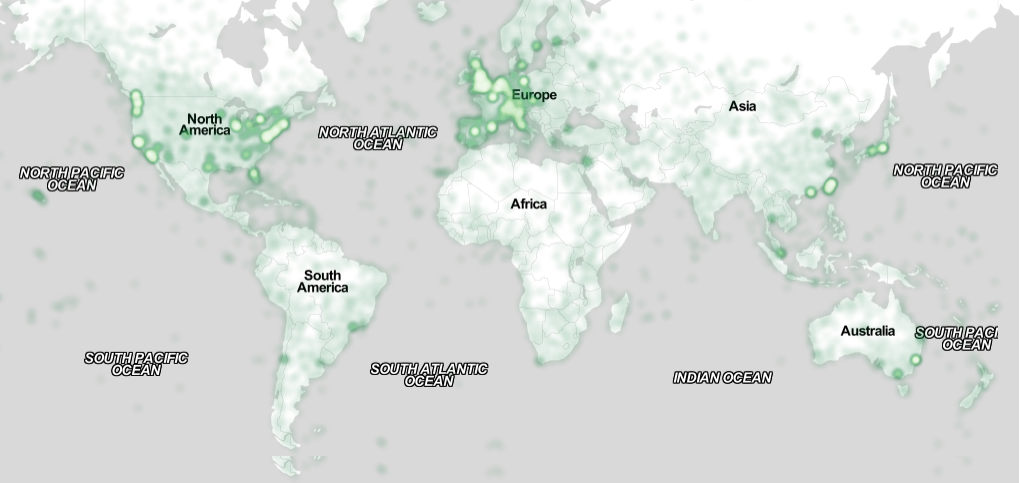
\includegraphics[width=1.75\columnwidth]{figures/map}
%   \caption{In this image, the map maximizes use of space. You can make
%     figures as wide as you need, up to a maximum of the full width of
%     both columns. Note that \LaTeX\ tends to render large figures on a
%     dedicated page. Image: \ccbynd~ayman on
%     Flickr.}~\label{fig:figure2}
% \end{figure*}


% \begin{itemize}
% \item Write in a straightforward style.
% \item Try to avoid long or complex sentence structures.
% \item Briefly define or explain all technical terms that may be
%   unfamiliar to readers.
% \item Explain all acronyms the first time they are used in your
%   text---e.g., ``Digital Signal Processing (DSP)''.
% \item Explain local references (e.g., not everyone knows all city
%   names in a particular country).
% \item Explain ``insider'' comments. Ensure that your whole audience
%   understands any reference whose meaning you do not describe (e.g.,
%   do not assume that everyone has used a Macintosh or a particular
%   application).
% \item Explain colloquial language and puns. Understanding phrases like
%   ``red herring'' may require a local knowledge of English.  Humor and
%   irony are difficult to translate.
% \item Use unambiguous forms for culturally localized concepts, such as
%   times, dates, currencies, and numbers (e.g., ``1--5--97'' or
%   ``5/1/97'' may mean 5 January or 1 May, and ``seven o'clock'' may
%   mean 7:00 am or 19:00). For currencies, indicate equivalences:
%   ``Participants were paid {\fontfamily{txr}\selectfont \textwon}
%   25,000, or roughly US \$22.''
% \item Be careful with the use of gender-specific pronouns (he, she)
%   and other gendered words (chairman, manpower, man-months). Use
%   inclusive language that is gender-neutral (e.g., she or he, they,
%   s/he, chair, staff, staff-hours, person-years). See the
%   \textit{Guidelines for Bias-Free Writing} for further advice and
%   examples regarding gender and other personal
%   attributes~\cite{Schwartz:1995:GBF}. Be particularly aware of
%   considerations around writing about people with disabilities.
% \item If possible, use the full (extended) alphabetic character set
%   for names of persons, institutions, and places (e.g.,
%   Gr{\o}nb{\ae}k, Lafreni\'ere, S\'anchez, Nguy{\~{\^{e}}}n,
%   Universit{\"a}t, Wei{\ss}enbach, Z{\"u}llighoven, \r{A}rhus, etc.).
%   These characters are already included in most versions and variants
%   of Times, Helvetica, and Arial fonts.
% \end{itemize}

% Balancing columns in a ref list is a bit of a pain because you
% either use a hack like flushend or balance, or manually insert
% a column break.  http://www.tex.ac.uk/cgi-bin/texfaq2html?label=balance
% multicols doesn't work because we're already in two-column mode,
% and flushend isn't awesome, so I choose balance.  See this
% for more info: http://cs.brown.edu/system/software/latex/doc/balance.pdf
%
% Note that in a perfect world balance wants to be in the first
% column of the last page.
%
% If balance doesn't work for you, you can remove that and
% hard-code a column break into the bbl file right before you
% submit:
%
% http://stackoverflow.com/questions/2149854/how-to-manually-equalize-columns-
% in-an-ieee-paper-if-using-bibtex
%
% Or, just remove \balance and give up on balancing the last page.
%
\balance{}

\section{References Format}
Your references should be published materials accessible to the
public. Internal technical reports may be cited only if they are
easily accessible and may be obtained by any reader for a nominal
fee. Proprietary information may not be cited. Private communications
should be acknowledged in the main text, not referenced (e.g.,
[Golovchinsky, personal communication]). References must be the same
font size as other body text. References should be in alphabetical
order by last name of first author. Use a numbered list of references
at the end of the article, ordered alphabetically by last name of
first author, and referenced by numbers in brackets. For papers from
conference proceedings, include the title of the paper and the name of
the conference. Do not include the location of the conference or the
exact date; do include the page numbers if available. 

References should be in ACM citation format:
\url{http://www.acm.org/publications/submissions/latex_style}.  This
includes citations to Internet
resources~\cite{CHINOSAUR:venue,cavender:writing,psy:gangnam}
according to ACM format, although it is often appropriate to include
URLs directly in the text, as above. Example reference formatting for
individual journal articles~\cite{ethics}, articles in conference
proceedings~\cite{Klemmer:2002:WSC:503376.503378},
books~\cite{Schwartz:1995:GBF}, theses~\cite{sutherland:sketchpad},
book chapters~\cite{winner:politics}, an entire journal
issue~\cite{kaye:puc},
websites~\cite{acm_categories,cavender:writing},
tweets~\cite{CHINOSAUR:venue}, patents~\cite{heilig:sensorama}, 
games~\cite{supermetroid:snes}, and
online videos~\cite{psy:gangnam} is given here.  See the examples of
citations at the end of this document and in the accompanying
\texttt{BibTeX} document. This formatting is a edited version of the
format automatically generated by the ACM Digital Library
(\url{http://dl.acm.org}) as ``ACM Ref.'' DOI and/or URL links are
optional but encouraged as are full first names. Note that the
Hyperlink style used throughout this document uses blue links;
however, URLs in the references section may optionally appear in
black.

% BALANCE COLUMNS
\balance{}

% REFERENCES FORMAT
% References must be the same font size as other body text.
\bibliographystyle{SIGCHI-Reference-Format}
\bibliography{sample}

\end{document}

%%% Local Variables:
%%% mode: latex
%%% TeX-master: t
%%% End:
